% ── Chapter 4: Results and Discussion ────────────────────────

\chapter{Results and Discussion}

This chapter presents the experimental results obtained from the two
principal subsystems of the proposed framework. Section~\ref{sec:nav}
presents the quantitative performance evaluation of vision-based
autonomous path following. Section~\ref{sec:env} presents the
real-time sensor data acquisition, cloud transmission, and dashboard
results. Section~\ref{sec:disc} provides a consolidated discussion,
and Section~\ref{sec:lim} identifies the limitations of the current
implementation.

\section{Vision-Based Autonomous Path Following}
\label{sec:nav}

\subsection{Experimental Setup and Performance Metrics}

All path-following experiments were conducted on a closed rectangular
trajectory of 152.4\,cm $\times$ 91.44\,cm constructed using red
adhesive tape on a tiled indoor floor, with a total perimeter of
487.68\,cm. Figure~\ref{fig:robotpath} shows the experimental path.
A total of 40 trials were performed: 20 under manual teleoperation
and 20 under autonomous vision-based navigation, under identical
lighting and environmental conditions.

\begin{figure}[tbp]
  \centering
  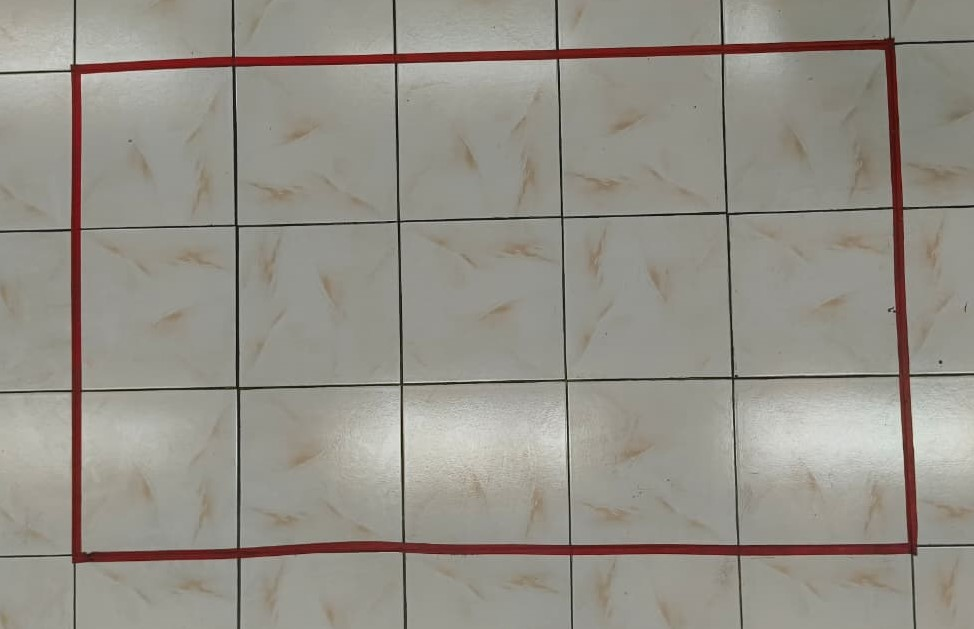
\includegraphics[width=0.82\textwidth]{WhatsApp Image 2026-04-10 at 1.09.01 PM (2).jpeg}
  \caption{Rectangular red tape path on tiled floor used for all 40 experimental trials.}
  \label{fig:robotpath}
\end{figure}

The primary performance metric is the Root Mean Square Error (RMSE)
of lateral deviation. The RMSE is a standard measure of tracking
accuracy in mobile robot navigation, and is computed per trial as
given in Equation~\eqref{eq:rmse}:

\begin{equation}
  \text{RMSE} = \sqrt{\frac{1}{N}\sum_{i=1}^{N} e_i^2}
  \label{eq:rmse}
\end{equation}

\noindent where $e_i$ is the instantaneous lateral tracking error at
sample $i$ and $N$ is the total number of recorded samples.
The sample mean error and standard deviation of tracking errors are
defined in Equation~\eqref{eq:mean_std} as:

\begin{equation}
  \bar{e} = \frac{1}{N}\sum_{i=1}^{N} e_i, \qquad
  \sigma  = \sqrt{\frac{1}{N}\sum_{i=1}^{N}(e_i - \bar{e})^2}
  \label{eq:mean_std}
\end{equation}

\noindent where $\bar{e}$ is the sample mean and $\sigma$ the standard
deviation of the instantaneous lateral tracking errors across a trial.

The maximum possible lateral deviation, corresponding to half the path
width, is given in Equation~\eqref{eq:emax}:

\begin{equation}
  E_{\max} = \frac{W}{2} = \frac{91.44}{2} = 45.72\,\text{cm}
  \label{eq:emax}
\end{equation}

\noindent where $W$ is the physical path width in centimetres.
Using Equation~\eqref{eq:emax}, the normalised tracking error and
tracking accuracy are computed in Equation~\eqref{eq:accuracy} as:

\begin{equation}
  E_{\text{norm}} = \frac{\text{RMSE}}{E_{\max}}, \qquad
  \text{Accuracy} = 1 - E_{\text{norm}}
  \label{eq:accuracy}
\end{equation}

\noindent where tracking accuracy is expressed as the proportion of
the path width that the robot maintains.

\subsection{Trajectory Analysis and Descriptive Statistics}

Figure~\ref{fig:traj_best} presents the best-performing trial pair:
manual trial~18 (RMSE = 14.75\,cm) against autonomous run~19
(RMSE = 1.489\,cm). The manual trajectory shows noticeable outward
deviation at all four straight segments and corner transitions.
Autonomous run~19 stays remarkably close to the reference line
throughout the entire lap.

\begin{figure}[tbp]
  \centering
  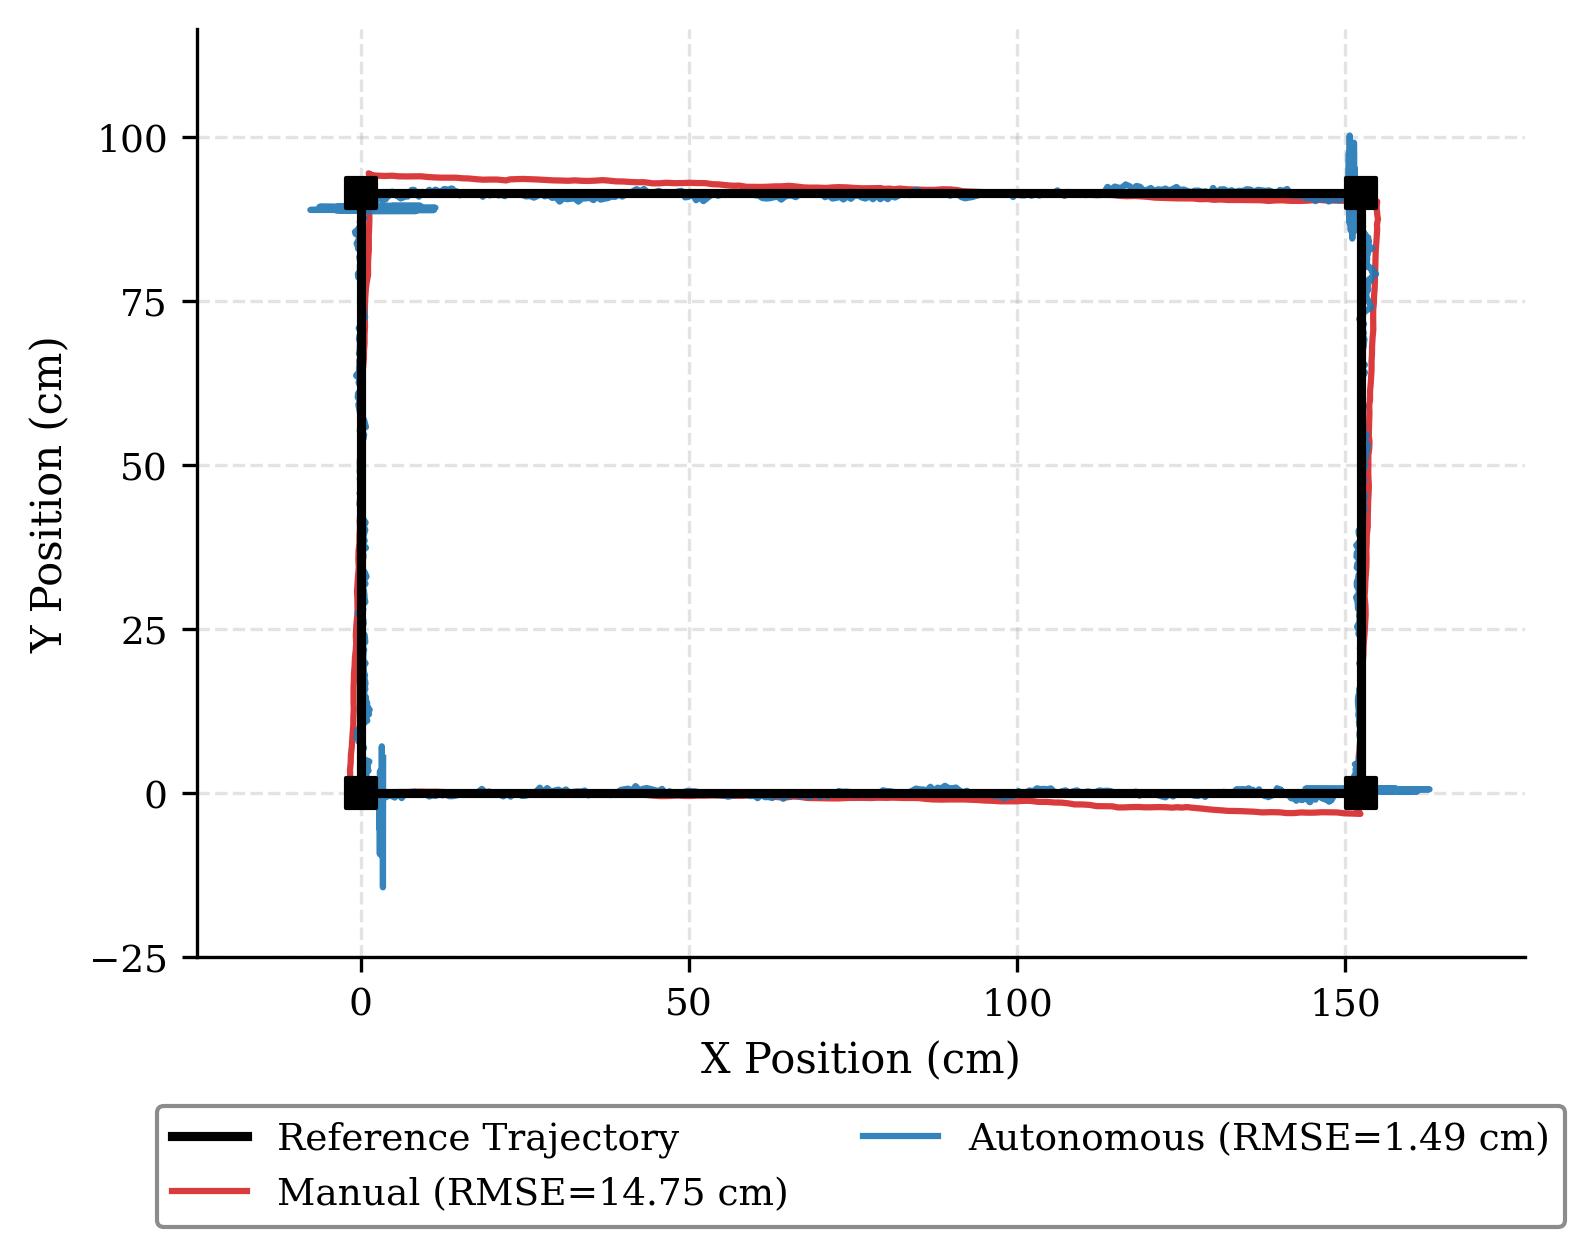
\includegraphics[width=0.90\textwidth]{plot_path_best.png}
  \caption{Best-case trajectory pair: manual trial~18 vs.\ autonomous run~19 overlaid on the reference path.}
  \label{fig:traj_best}
\end{figure}

Figure~\ref{fig:traj_worst} presents all 20 autonomous trajectories
overlaid on the reference path. Even the worst autonomous trial
(run~20, RMSE = 5.554\,cm) is considerably lower than the best manual
trial ever recorded (14.751\,cm), a difference of over 9\,cm, which
confirms that the two distributions do not overlap at all.

\begin{figure}[tbp]
  \centering
  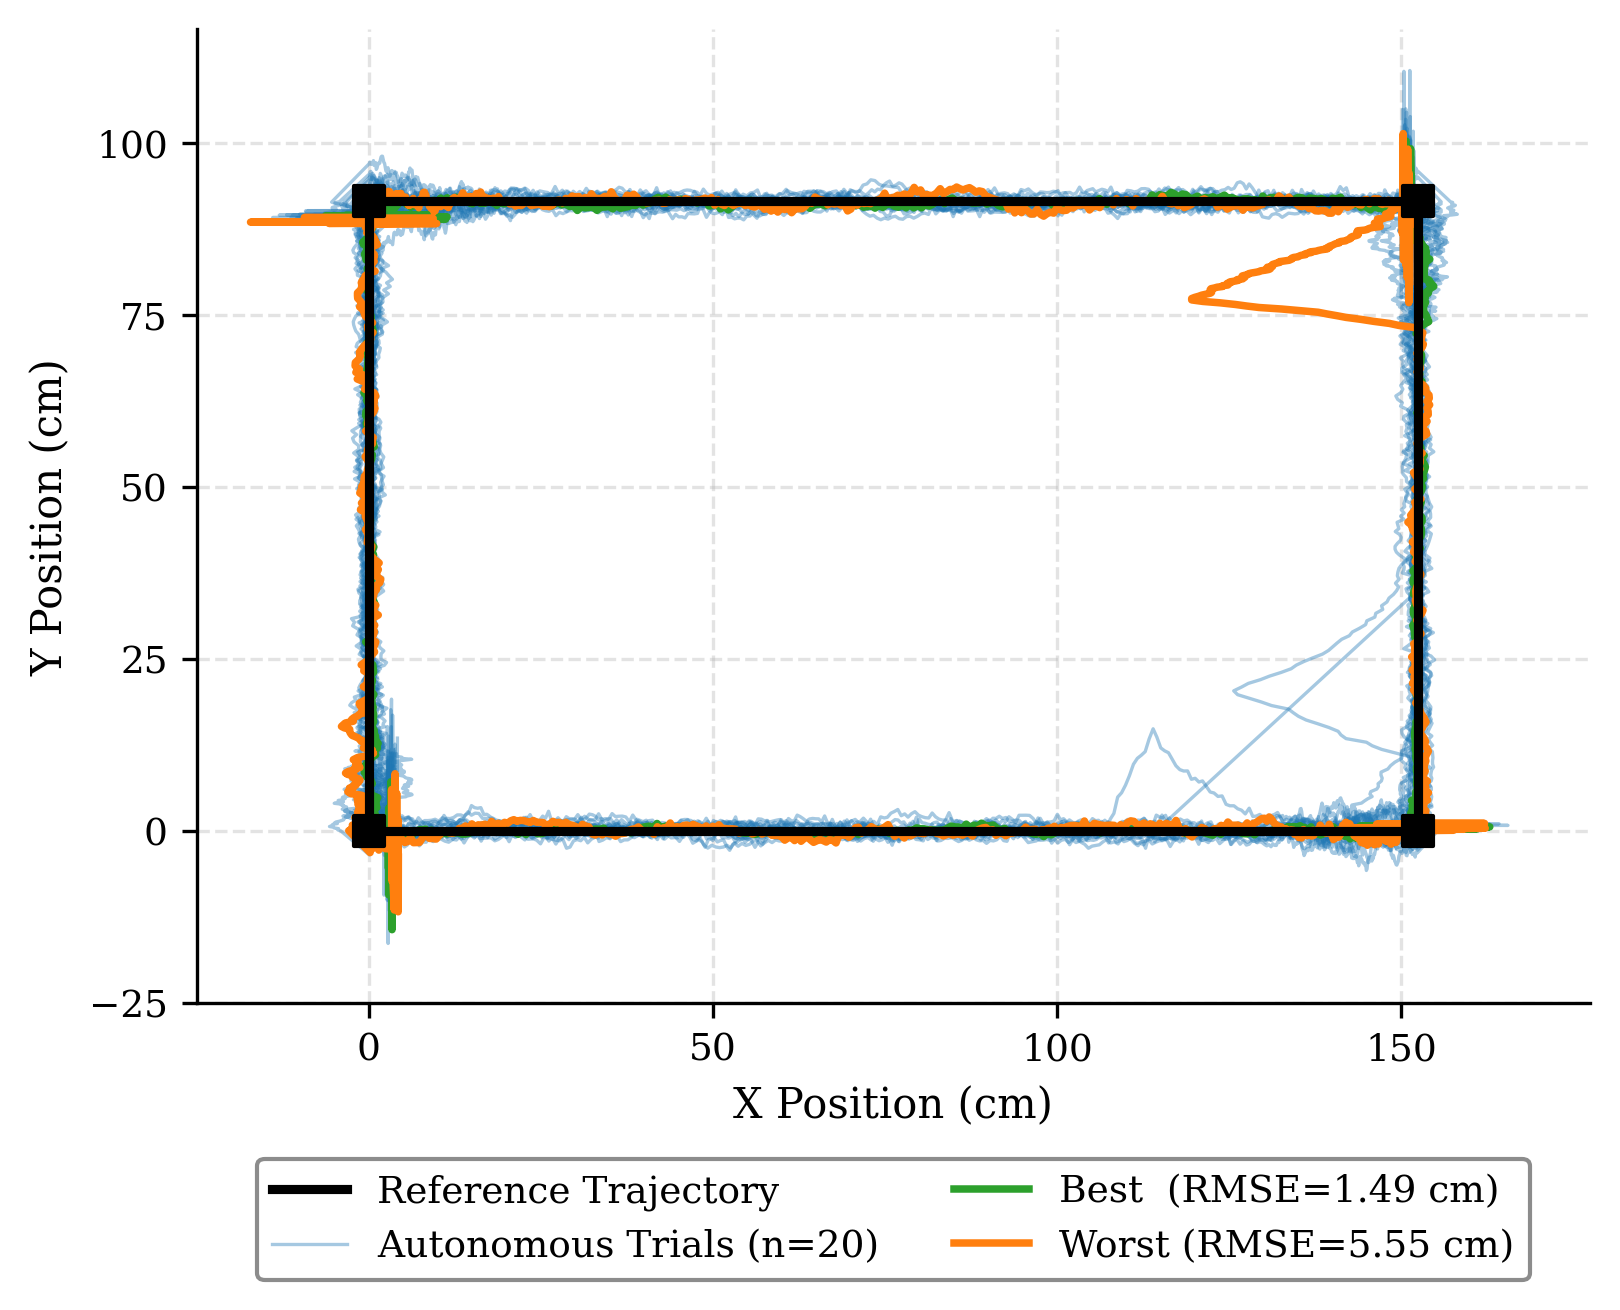
\includegraphics[width=0.90\textwidth]{plot_path_all_autonomous.png}
  \caption{All 20 autonomous trial trajectories overlaid on the reference path. The worst autonomous trial (run~20, 5.55\,cm) remains below the best manual trial (14.75\,cm).}
  \label{fig:traj_worst}
\end{figure}

Table~\ref{tab:desc_stats} presents the per-trial RMSE summary
statistics. The autonomous mode achieves a mean RMSE of 2.222\,cm,
an 86.75\% reduction from the manual mean of 16.768\,cm.
Even the worst 5\% of autonomous trials (95th percentile = 4.087\,cm)
fell well below the best manual trial ever recorded (14.751\,cm),
demonstrating consistent superiority of closed-loop autonomous
control over manual teleoperation.

\begin{table}[tbp]
  \centering
  \caption{Per-trial RMSE descriptive statistics for both operating modes ($n=20$, values in cm).}
  \label{tab:desc_stats}
  \begin{tabular}{lcccc}
    \toprule
    Metric          & Manual & Autonomous & Reduction & Reduction (\%) \\
    \midrule
    Mean RMSE       & 16.768 & 2.222      & 14.546    & 86.75\% \\
    Median RMSE     & 16.211 & 1.980      & 14.231    & 87.8\%  \\
    Std Deviation   & 2.101  & 0.958      & 1.143     & 54.4\%  \\
    Minimum         & 14.751 & 1.489      & 13.262    & --      \\
    Maximum         & 23.147 & 5.554      & 17.593    & 76.0\%  \\
    95th Percentile & 19.969 & 4.087      & 15.882    & 79.5\%  \\
    \bottomrule
    \multicolumn{5}{l}{\small $n = 20$ trials each $|$ 5\,ft $\times$ 3\,ft Rectangular Path}
  \end{tabular}
\end{table}

\subsection{Temporal Error Behaviour and Error Distribution}

Figure~\ref{fig:rmse_bar} presents the per-trial RMSE values for all
40 trials. Manual RMSE values range from 14.751\,cm to 23.147\,cm.
Autonomous RMSE values are consistently low, ranging from 1.365\,cm
to 5.588\,cm across all 20 trials, with no overlap between the two
distributions.

\begin{figure}[tbp]
  \centering
  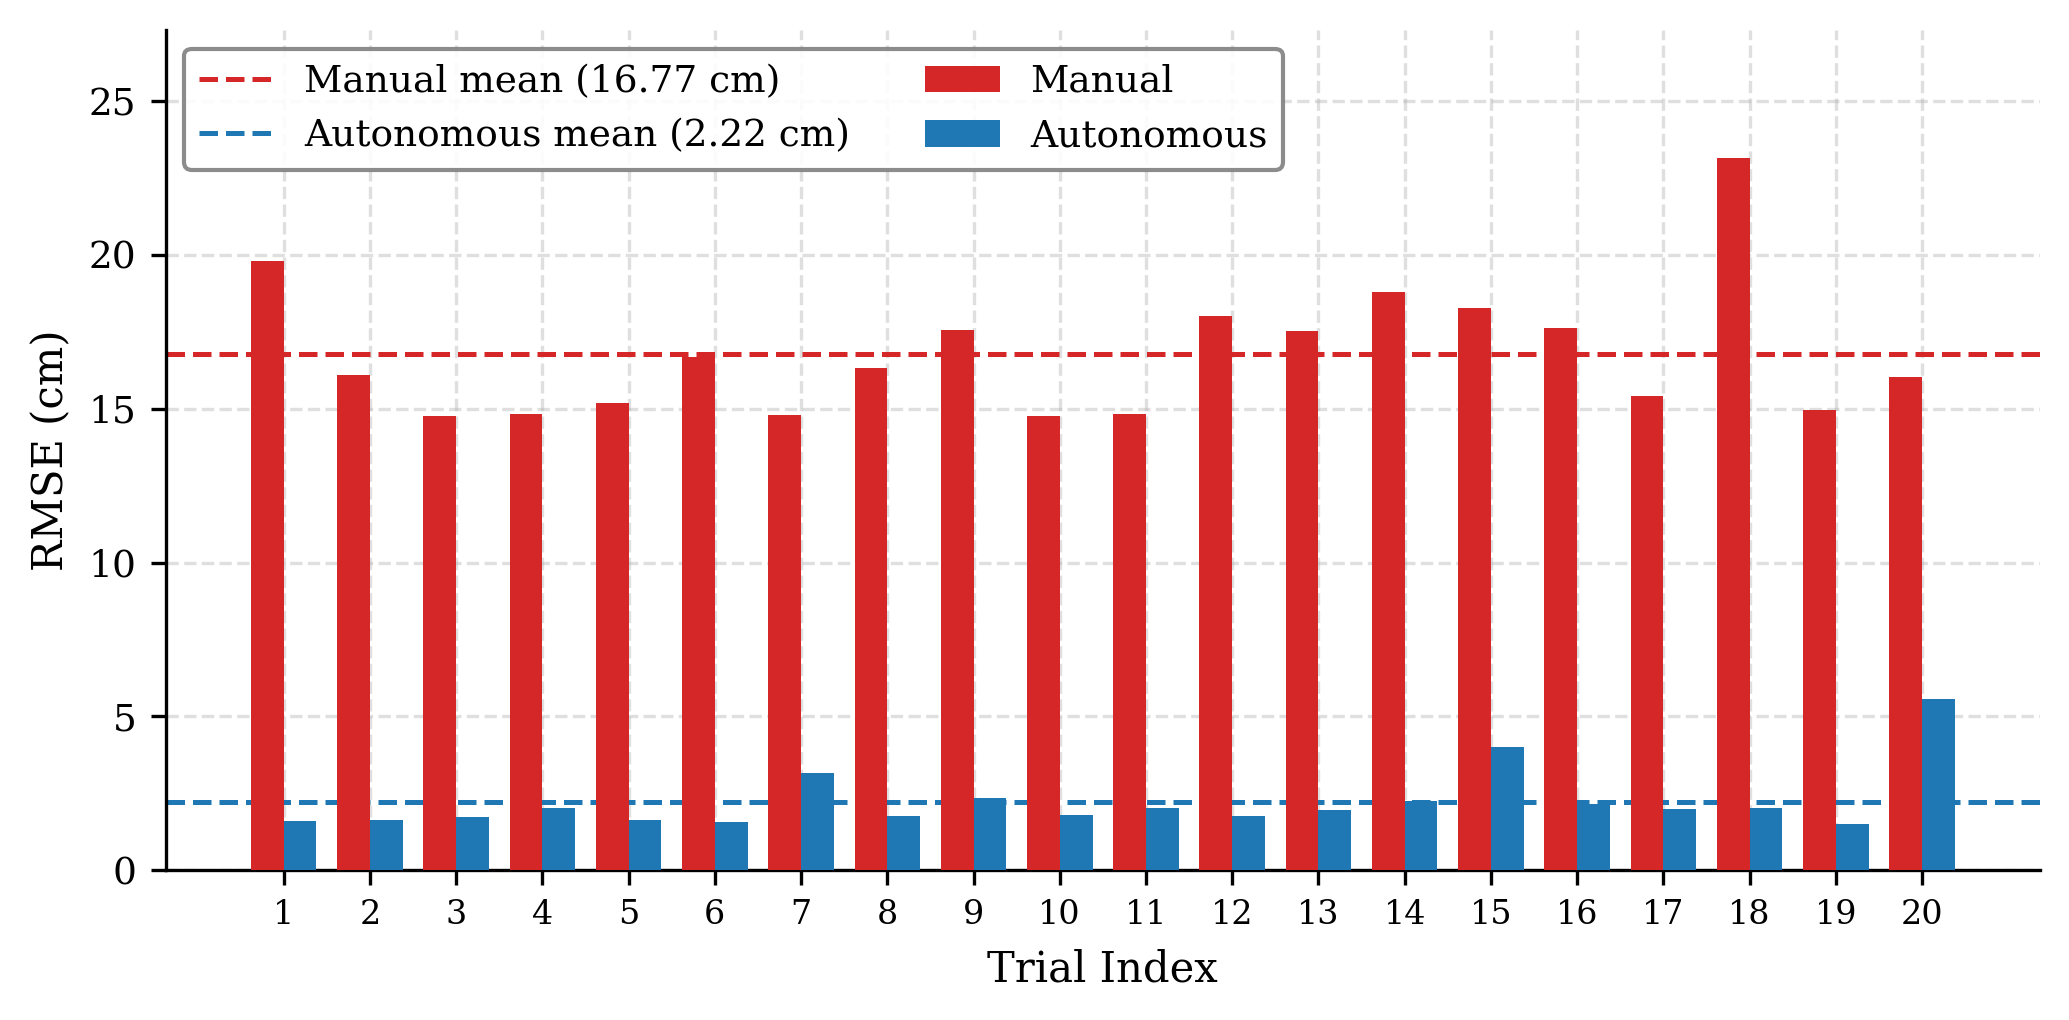
\includegraphics[width=0.88\textwidth]{plot_per_trial_rmse_bar.png}
  \caption{Per-trial RMSE for all 20 manual and 20 autonomous trials. No autonomous trial exceeds 5.55\,cm; no manual trial falls below 14.75\,cm.}
  \label{fig:rmse_bar}
\end{figure}

Figure~\ref{fig:error_time} shows the temporal evolution of tracking
error for the best trial in each mode. The manual trace fluctuates
within approximately 10 to 16\,cm. The autonomous trace maintains
near-zero error throughout all four straight segments with narrow
spikes only at corner transitions, confirming the effectiveness of
the PID derivative term in damping rapid deviation changes.

\begin{figure}[tbp]
  \centering
  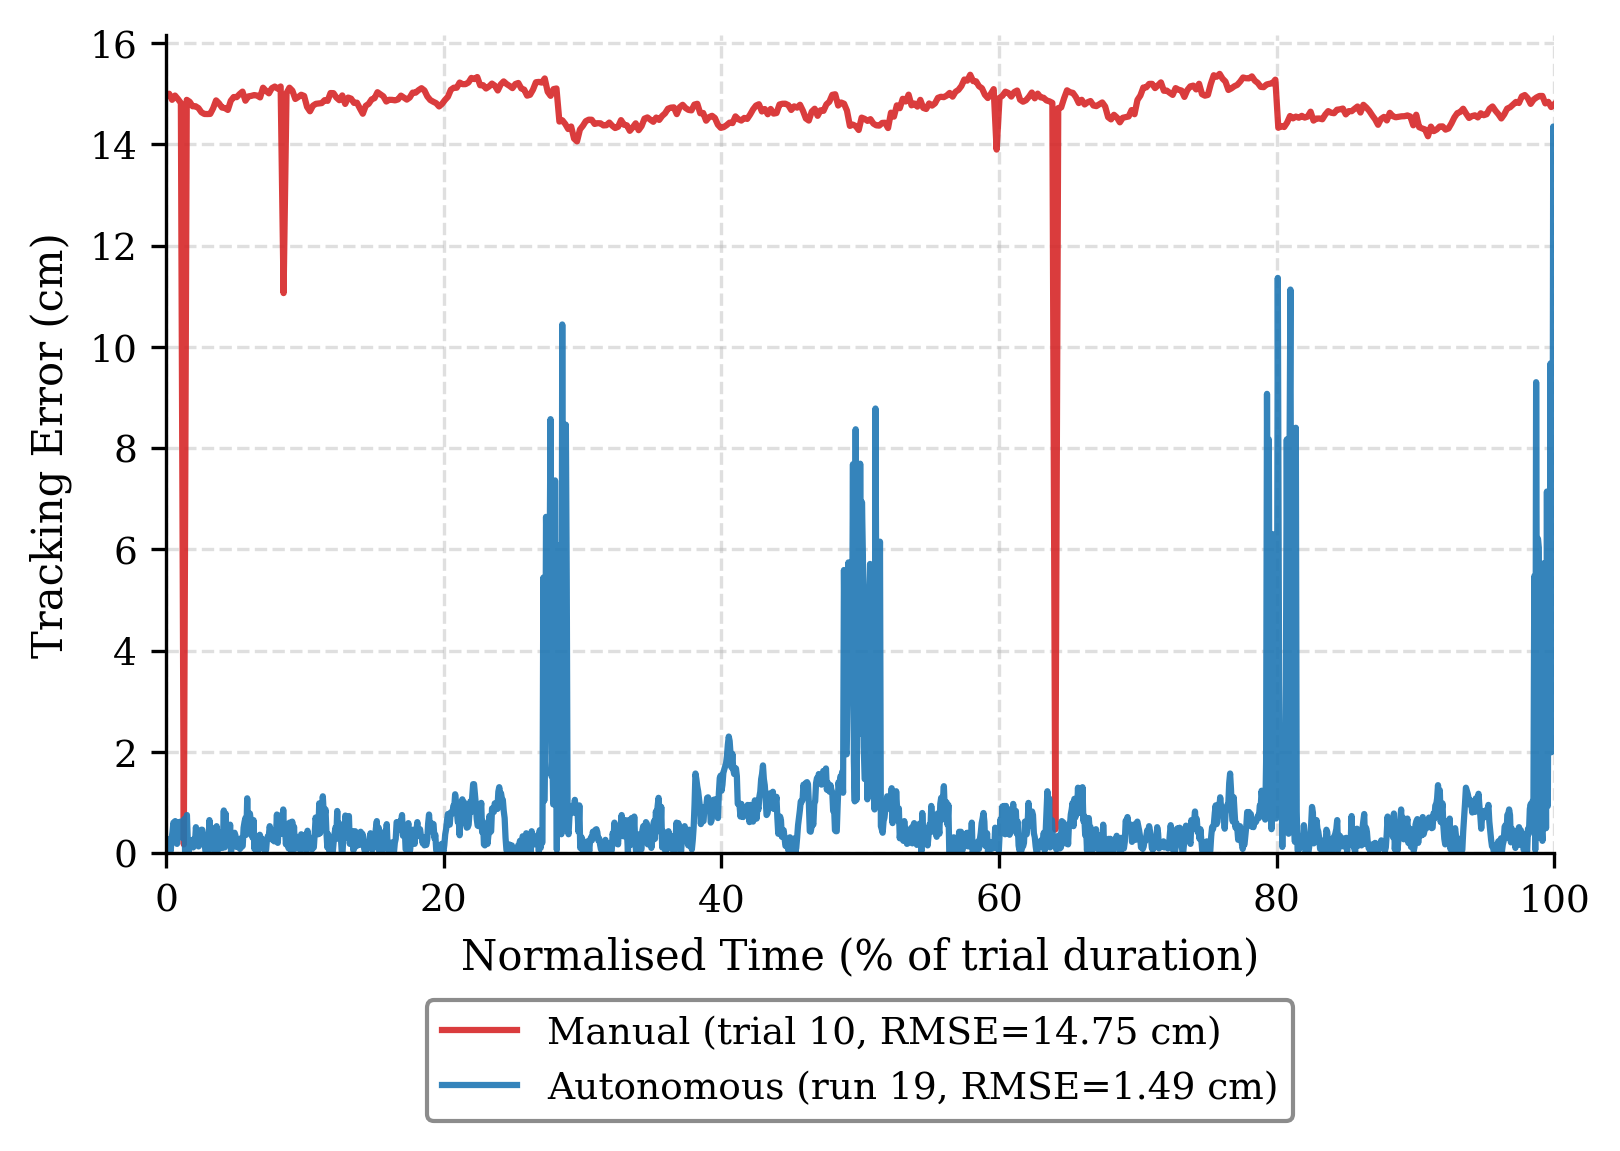
\includegraphics[width=0.88\textwidth]{plot_error_over_time_best.png}
  \caption{Tracking error over normalised trial time for the best manual (trial~18) and best autonomous (run~19) trial.}
  \label{fig:error_time}
\end{figure}

Figure~\ref{fig:histogram} presents the probability distribution of
instantaneous tracking errors. The manual distribution is broad,
centred near 15\,cm. The autonomous distribution is narrow and sharply
peaked near 0\,cm, confirming systematic improvement.

\begin{figure}[tbp]
  \centering
  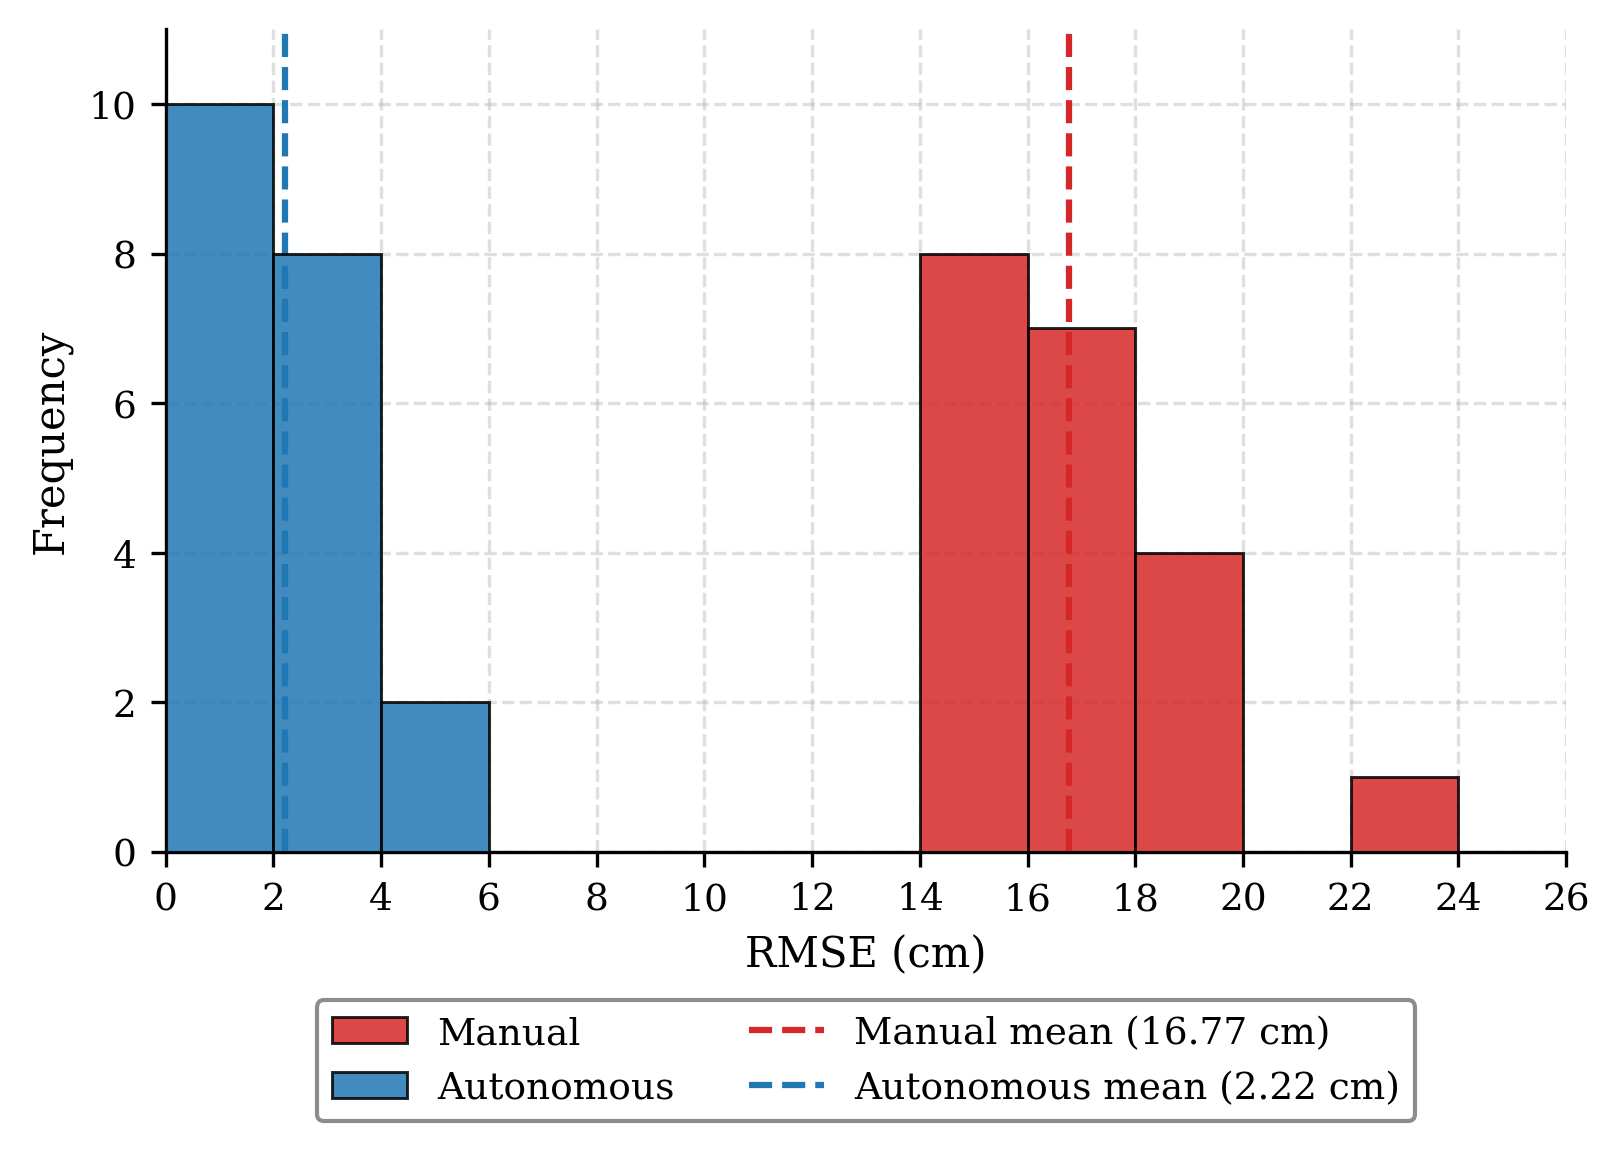
\includegraphics[width=0.85\textwidth]{plot_histogram.png}
  \caption{Probability distribution of instantaneous tracking errors for manual and autonomous modes.}
  \label{fig:histogram}
\end{figure}

Figure~\ref{fig:cdf} presents the cumulative distribution function
of per-trial RMSE for both modes. The autonomous distribution rises
steeply and reaches its maximum at 5.588\,cm, well before the manual
distribution begins to rise from 14.751\,cm, demonstrating complete
stochastic dominance of autonomous over manual performance.

\begin{figure}[tbp]
  \centering
  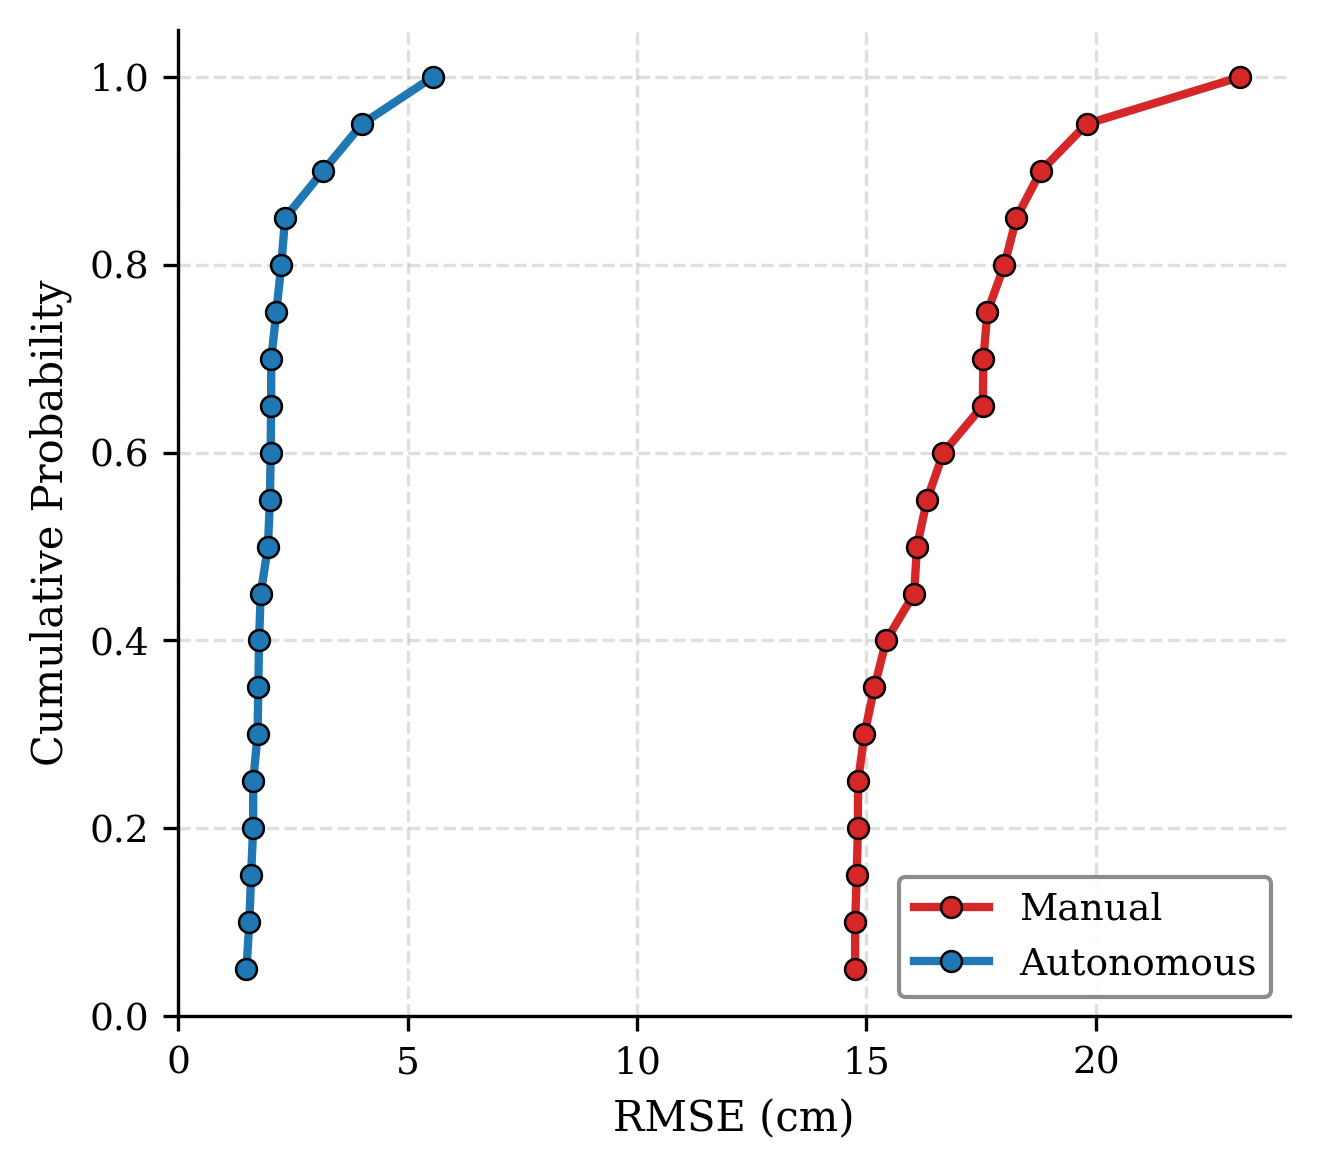
\includegraphics[width=0.82\textwidth]{plot_cdf.png}
  \caption{Cumulative distribution function of per-trial RMSE for manual and autonomous modes, showing complete stochastic dominance of autonomous over manual.}
  \label{fig:cdf}
\end{figure}

\subsection{Accuracy Analysis}

Using Equation~\eqref{eq:accuracy}, Table~\ref{tab:accuracy} presents
the tracking accuracy results. The autonomous mode achieves a mean
tracking accuracy of 95.14\%, compared with 63.33\% for manual
teleoperation, a gain of 31.81 percentage points.

\begin{table}[tbp]
  \centering
  \caption{Tracking accuracy analysis ($E_{\max} = 45.72$\,cm, $n=20$ each).}
  \label{tab:accuracy}
  \begin{tabular}{lcccc}
    \toprule
    Mode       & Mean RMSE (cm) & Norm.\ Error & Accuracy (\%) & Gain \\
    \midrule
    Manual     & 16.768         & 0.3668       & 63.33\%       & --       \\
    Autonomous & 2.222          & 0.0486       & 95.14\%       & +31.81\% \\
    \bottomrule
  \end{tabular}
\end{table}

\subsection{Statistical Validation}

The statistical analysis proceeds in four stages. The results are
presented below in order of normality testing, hypothesis testing,
effect size measurement, and bootstrap confidence interval estimation.

\paragraph{Normality Testing.}
The Shapiro--Wilk test was applied to both distributions
to determine whether parametric or non-parametric tests are appropriate.
Table~\ref{tab:normality} confirms that both distributions are
non-normal ($p < 0.05$), justifying the use of non-parametric tests.

\begin{table}[tbp]
  \centering
  \caption{Shapiro--Wilk normality test results for per-trial RMSE.}
  \label{tab:normality}
  \begin{tabular}{lcccc}
    \toprule
    Mode       & $W$    & $p$-value & Normal?         & Action \\
    \midrule
    Manual     & 0.8502 & 0.0054    & No ($p < 0.05$) & Non-parametric test \\
    Autonomous & 0.6564 & 0.000012  & No ($p < 0.05$) & Non-parametric test \\
    \bottomrule
  \end{tabular}
\end{table}

\paragraph{Significance Testing.}
Table~\ref{tab:significance} presents four independent hypothesis
tests for $H_0$: Manual RMSE $\leq$ Autonomous RMSE versus $H_1$:
Manual RMSE $>$ Autonomous RMSE. All four tests unanimously reject
$H_0$ with $p$-values many orders of magnitude below the conventional
threshold of $\alpha = 0.05$.

\begin{table}[tbp]
  \centering
  \caption{Significance testing results ($H_1$: Manual RMSE $>$ Autonomous RMSE).}
  \label{tab:significance}
  \resizebox{\textwidth}{!}{%
  \begin{tabular}{lcccc}
    \toprule
    Test                       & Statistic           & $p$-value            & Threshold       & Decision     \\
    \midrule
    Mann--Whitney U            & $U = 400$           & $6.80\times10^{-8}$  & $\alpha = 0.05$ & Reject $H_0$ \\
    Welch $t$-test             & $t = 27.46$         & $4.84\times10^{-21}$ & $\alpha = 0.05$ & Reject $H_0$ \\
    Paired $t$-test            & $t = 27.56$         & $8.77\times10^{-17}$ & $\alpha = 0.05$ & Reject $H_0$ \\
    Kolmogorov--Smirnov        & $D = 1.00$          & $1.45\times10^{-11}$ & $\alpha = 0.05$ & Reject $H_0$ \\
    \bottomrule
  \end{tabular}}
\end{table}

\paragraph{Effect Size Analysis.}
Table~\ref{tab:effect} presents multiple effect size measures.
Cohen's $d = 8.911$ places the result firmly in the ``exceptionally
large'' category. The rank-biserial correlation of $-1.0$
indicates that every single autonomous trial outperformed every single
manual trial, with no overlap whatsoever. The probability of superiority
of 100\% confirms near-certain dominance of autonomous navigation.

\begin{table}[tbp]
  \centering
  \caption{Effect size measures for the performance difference between operating modes.}
  \label{tab:effect}
  \resizebox{\textwidth}{!}{%
  \begin{tabular}{lccc}
    \toprule
    Measure                      & Value            & Threshold (Large) & Classification \\
    \midrule
    Cohen's $d$                  & 8.911            & $d > 0.8$         & Exceptionally Large \\
    Rank-biserial $r$            & $-$1.000         & $|r| > 0.5$       & Perfect separation  \\
    Probability of Superiority   & 1.0000 (100.0\%) & $> 0.50$          & Near-certain superiority \\
    \bottomrule
  \end{tabular}}
\end{table}

\paragraph{Bootstrap Confidence Intervals.}
Table~\ref{tab:bootstrap} presents 95\% bootstrap confidence intervals
from 10,000 resampling iterations (seed = 42). The two
group intervals do not overlap. The mean improvement interval
$[13.21,\,15.90]$\,cm sits entirely above zero, ruling out any
possibility that the autonomous mode performs worse.

\begin{table}[tbp]
  \centering
  \caption{Bootstrap 95\% confidence intervals for mean RMSE (10,000 iterations).}
  \label{tab:bootstrap}
  \begin{tabular}{lccc}
    \toprule
    Quantity             & Observed   & 95\% CI Lower & 95\% CI Upper \\
    \midrule
    Manual Mean RMSE     & 16.768\,cm & 15.913\,cm    & 17.761\,cm    \\
    Autonomous Mean RMSE & 2.222\,cm  & 1.859\,cm     & 2.699\,cm     \\
    Difference (M $-$ A) & 14.547\,cm & 13.214\,cm    & 15.902\,cm    \\
    \bottomrule
  \end{tabular}
\end{table}

Figure~\ref{fig:violin} shows side-by-side violin plots with
box-and-whisker overlays. The violin width encodes probability density
at each RMSE level. The manual violin is wide and centred around
16\,cm; the autonomous violin is narrow and compact near 2\,cm. Their
interquartile ranges do not overlap: manual IQR spans
14.75--17.79\,cm while autonomous IQR spans 1.49--2.76\,cm.

\begin{figure}[tbp]
  \centering
  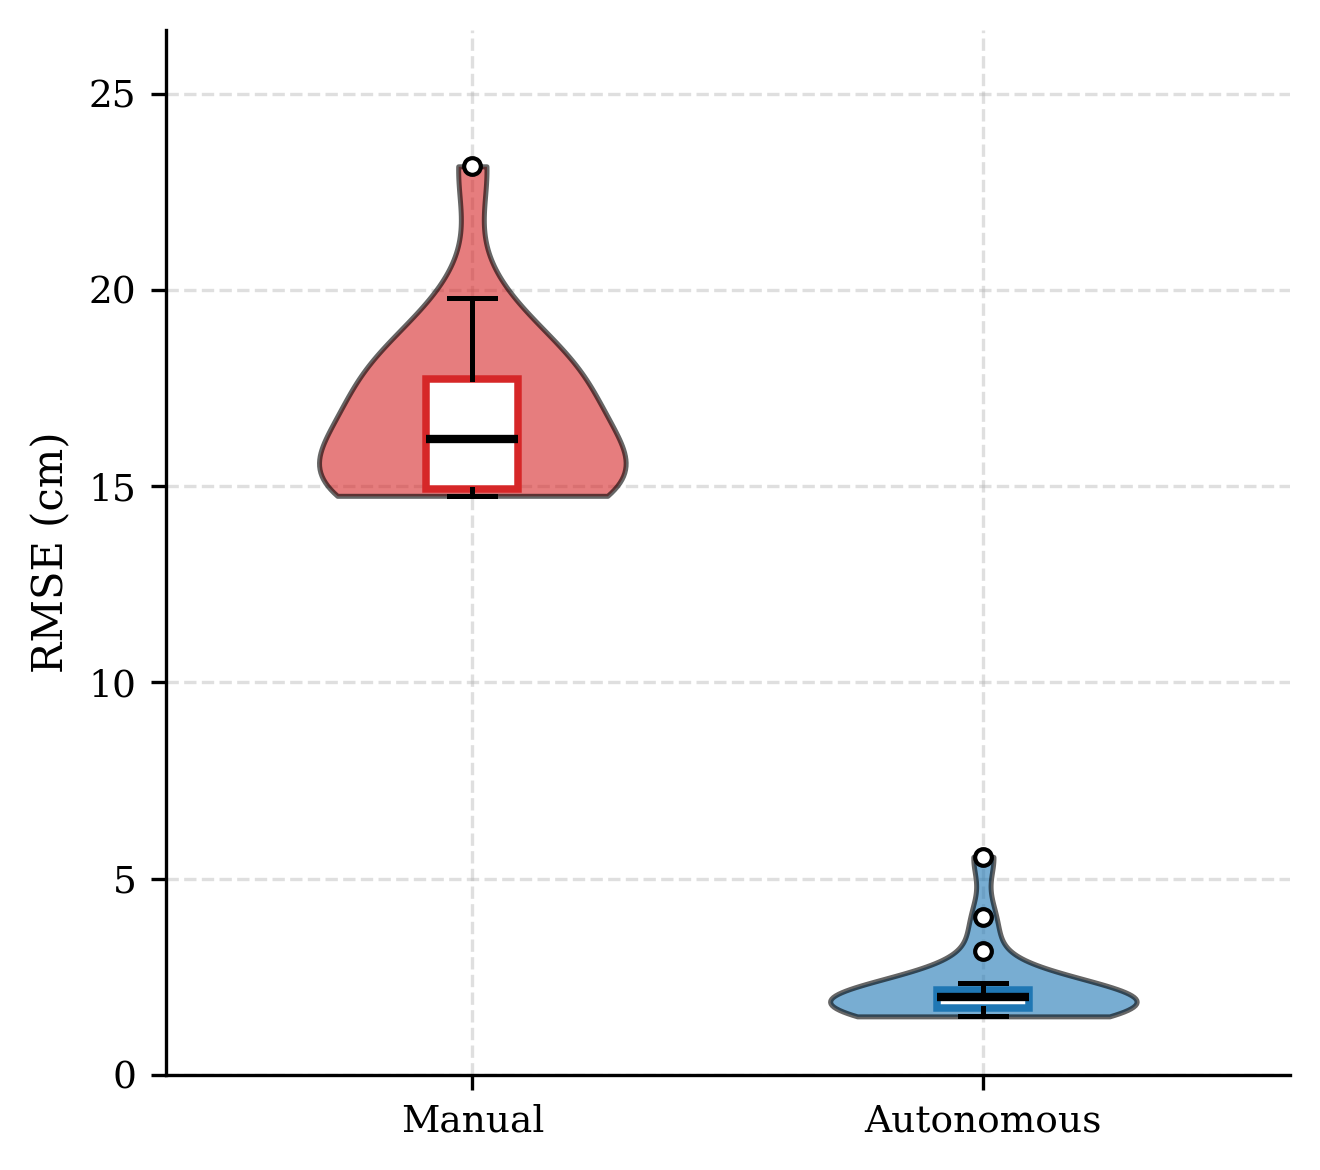
\includegraphics[width=0.85\textwidth]{plot_violin_box.png}
  \caption{Violin plots with box-and-whisker overlays for manual and autonomous RMSE distributions. The non-overlapping violins confirm complete distributional separation.}
  \label{fig:violin}
\end{figure}

% ─────────────────────────────────────────────────────────
\section{Environmental Monitoring System Results}
\label{sec:env}

\subsection{Sensor Data Acquisition, Local Storage, and Live Dashboard}

The environmental monitoring subsystem successfully acquired continuous
real-time measurements throughout all monitoring sessions. The SQLite
local database stored all readings with a 5-second acquisition cycle.
Figure~\ref{fig:sqlite} shows the SQLite database viewer
displaying the \texttt{readings} table with timestamped records beginning
from the first monitoring session on 2026-04-07. No write errors were
observed across any session.

\begin{figure}[tbp]
  \centering
  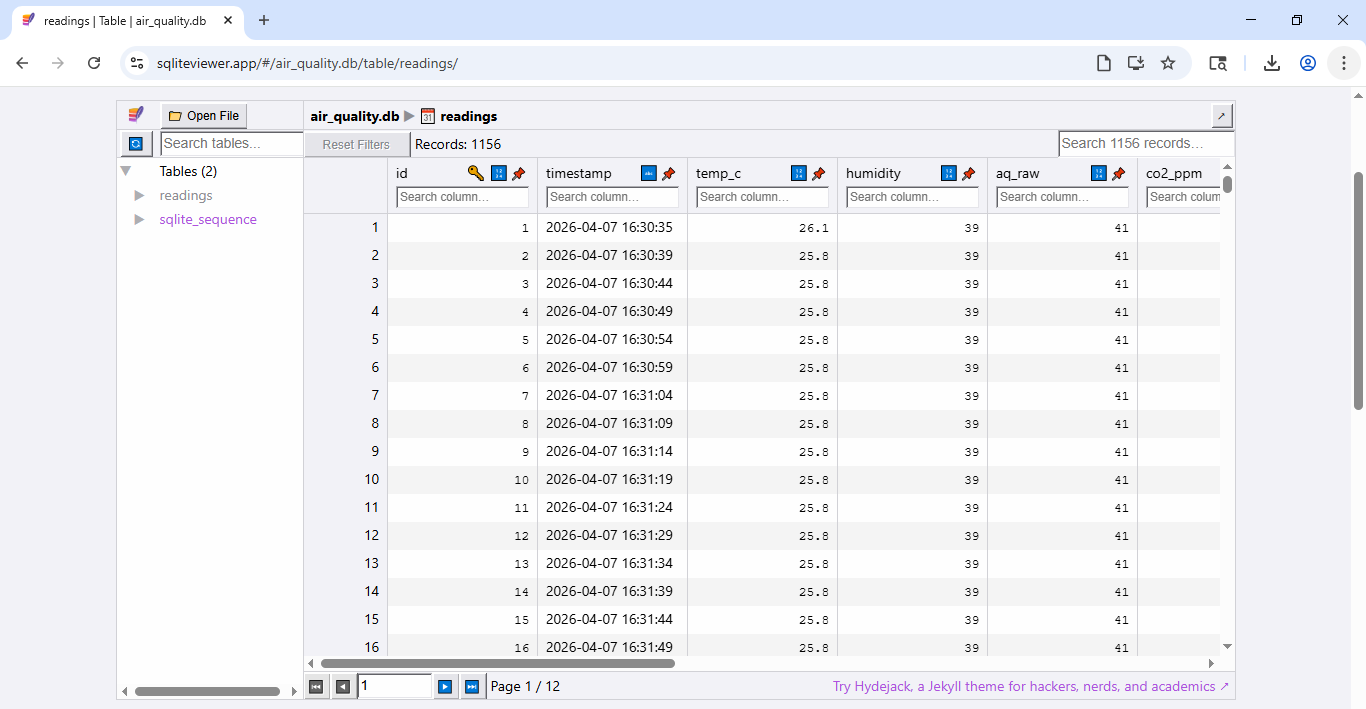
\includegraphics[width=0.95\textwidth]{sqlite3db.png}
  \caption{SQLite local database showing timestamped sensor records with temperature, humidity, raw AQ, and CO$_2$ fields.}
  \label{fig:sqlite}
\end{figure}

During the representative session on 2026-04-10, the system recorded
temperature of 27.1\,$^\circ$C, humidity of 39\%\,RH, raw MQ135 ADC
value of 40, and derived CO$_2$ of 357.03\,ppm, all classified as OK
according to the six-level alert scheme described in Chapter~3.

Figure~\ref{fig:flask1} shows the Flask live dashboard displaying four
metric tiles and three analogue gauge widgets with colour-coded zones.
The temperature gauge points to 27.1\,$^\circ$C within the green arc,
the humidity gauge reads 39\%\,RH, and the CO$_2$ gauge shows
357.03\,ppm well within the safe zone ($<$\,600\,ppm) as specified by
ASHRAE Standard~62.1.

\begin{figure}[tbp]
  \centering
  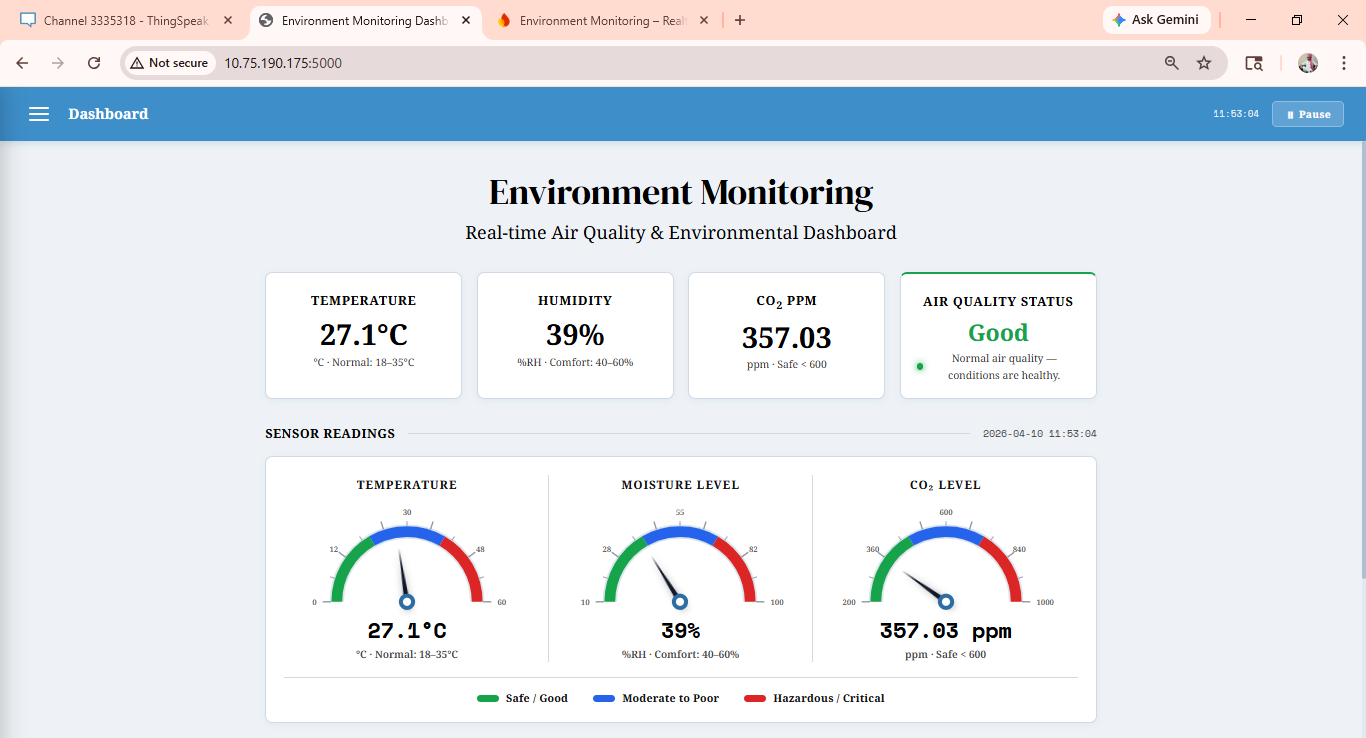
\includegraphics[width=0.90\textwidth]{Flask_Dashboard1.png}
  \caption{Flask live dashboard showing real-time temperature, humidity, and CO$_2$ gauge displays with air quality status.}
  \label{fig:flask1}
\end{figure}

Figure~\ref{fig:adv1} shows the Advanced Analysis view with the sensor
overview panel, system status cards, and environment status on the air
quality index scale, with the alert state confirmed as OK.

\begin{figure}[tbp]
  \centering
  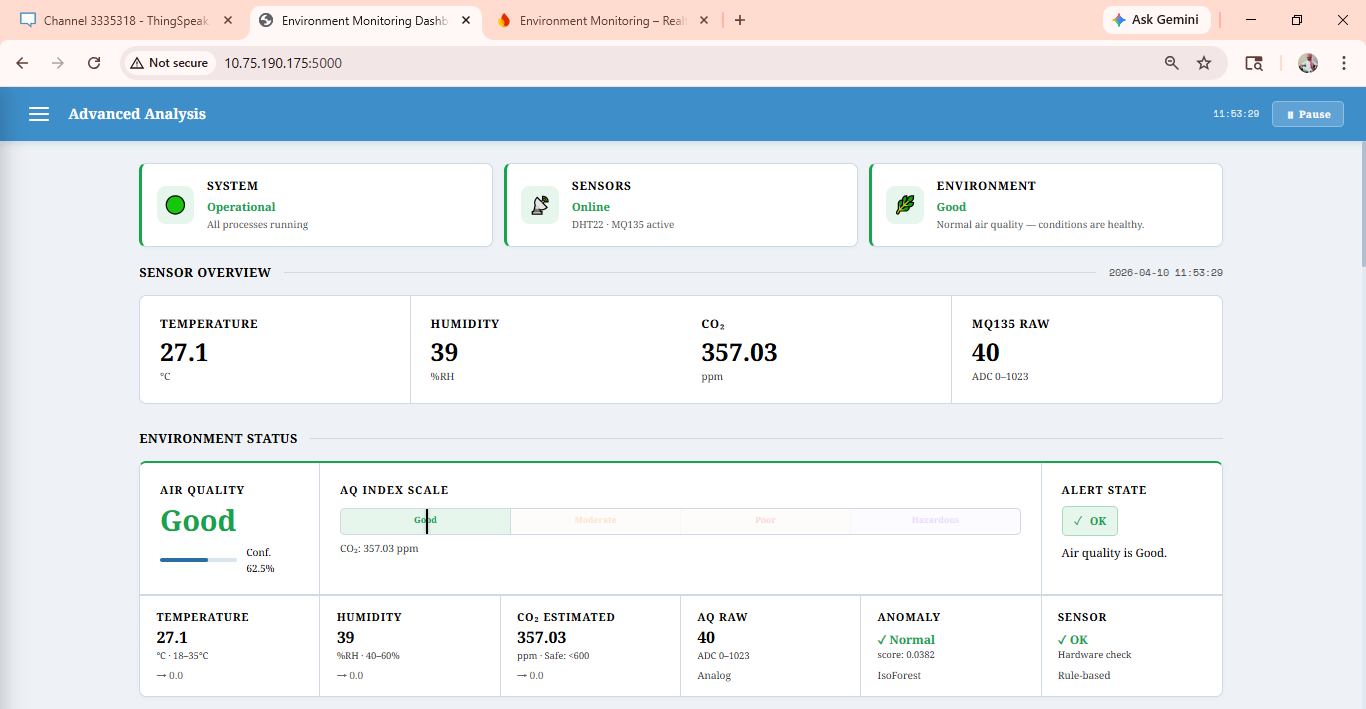
\includegraphics[width=0.90\textwidth]{Advanced_Analysis.png}
  \caption{Advanced Analysis dashboard showing sensor overview, system status, and air quality index scale.}
  \label{fig:adv1}
\end{figure}

Figure~\ref{fig:adv3} shows the CO$_2$ air quality trend with
colour-coded threshold bands aligned with established indoor air quality
standards. The CO$_2$ trace remains entirely within the
Good zone ($<$\,600\,ppm) throughout the session.

\begin{figure}[tbp]
  \centering
  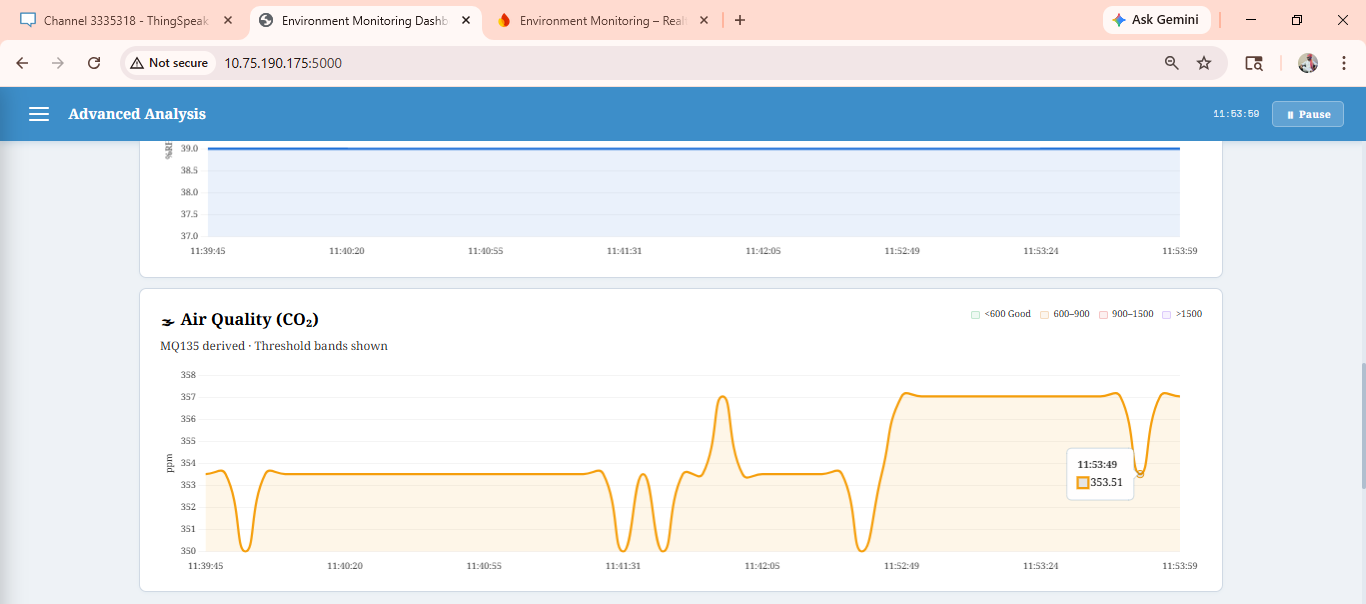
\includegraphics[width=0.90\textwidth]{Advanced_Analysis4.png}
  \caption{CO$_2$ air quality trend with threshold band overlay showing all readings within the Good zone.}
  \label{fig:adv3}
\end{figure}

\subsection{Cloud Transmission: Firebase and ThingSpeak}

Figure~\ref{fig:firebase} shows the Firebase Realtime Database console
hosted at the asia-southeast1 (Singapore) region. A
representative record in the \texttt{/readings} node contains:
\texttt{aq\_raw: 39}, \texttt{co2\_ppm: 353.51},
\texttt{humidity: 39}, \texttt{sensor\_fault: 0}, \texttt{temp\_c: 27.1}, and
\texttt{timestamp: ``2026-04-10 11:55:04''}. The background daemon
thread confirmed successful mirroring of all readings to the cloud
without blocking the acquisition loop.

\begin{figure}[tbp]
  \centering
  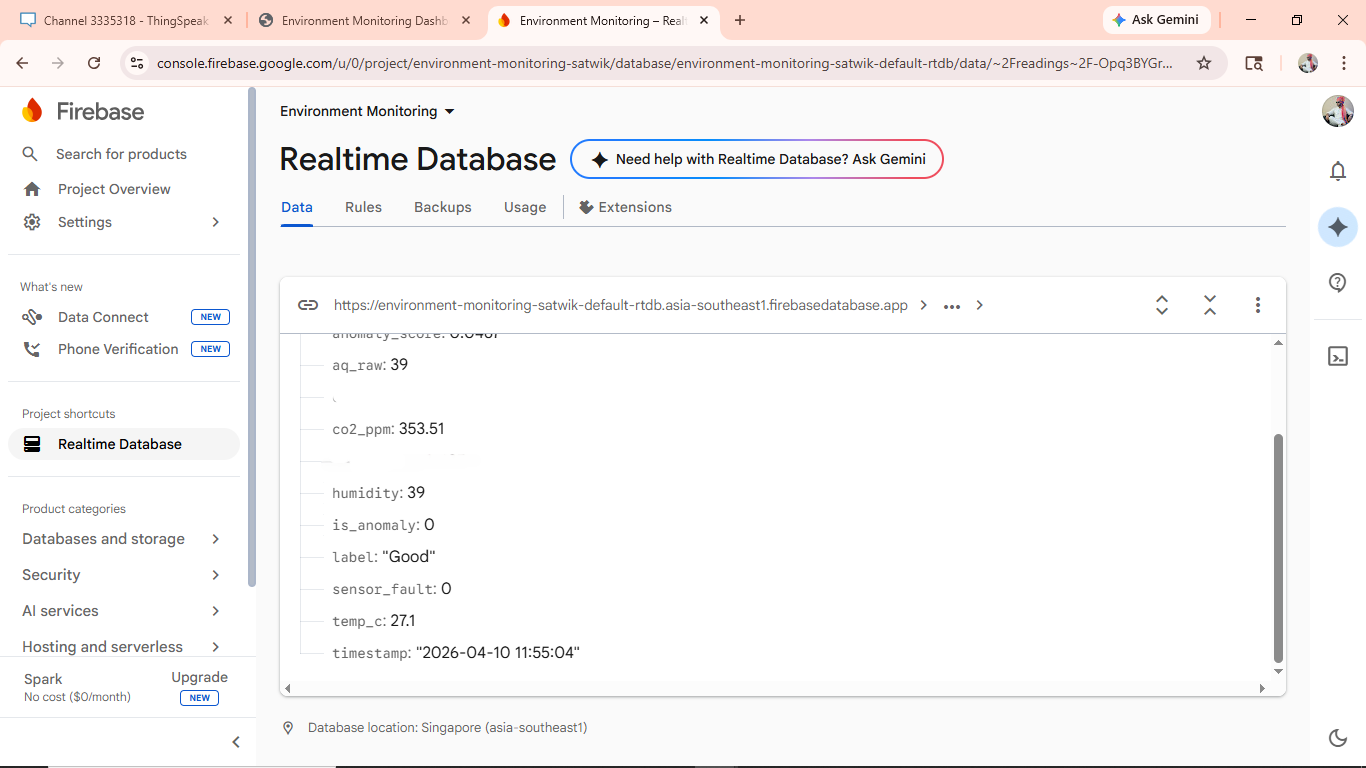
\includegraphics[width=0.90\textwidth]{Firebase1.png}
  \caption{Firebase Realtime Database console showing a stored sensor record with environmental fields.}
  \label{fig:firebase}
\end{figure}

Figure~\ref{fig:ts1} shows the ThingSpeak Channel 3335318 dashboard
with the Field 1 temperature gauge displaying 26.7\,$^\circ$C and the
CO$_2$ display showing 353.51\,ppm, confirming live transmission.

\begin{figure}[tbp]
  \centering
  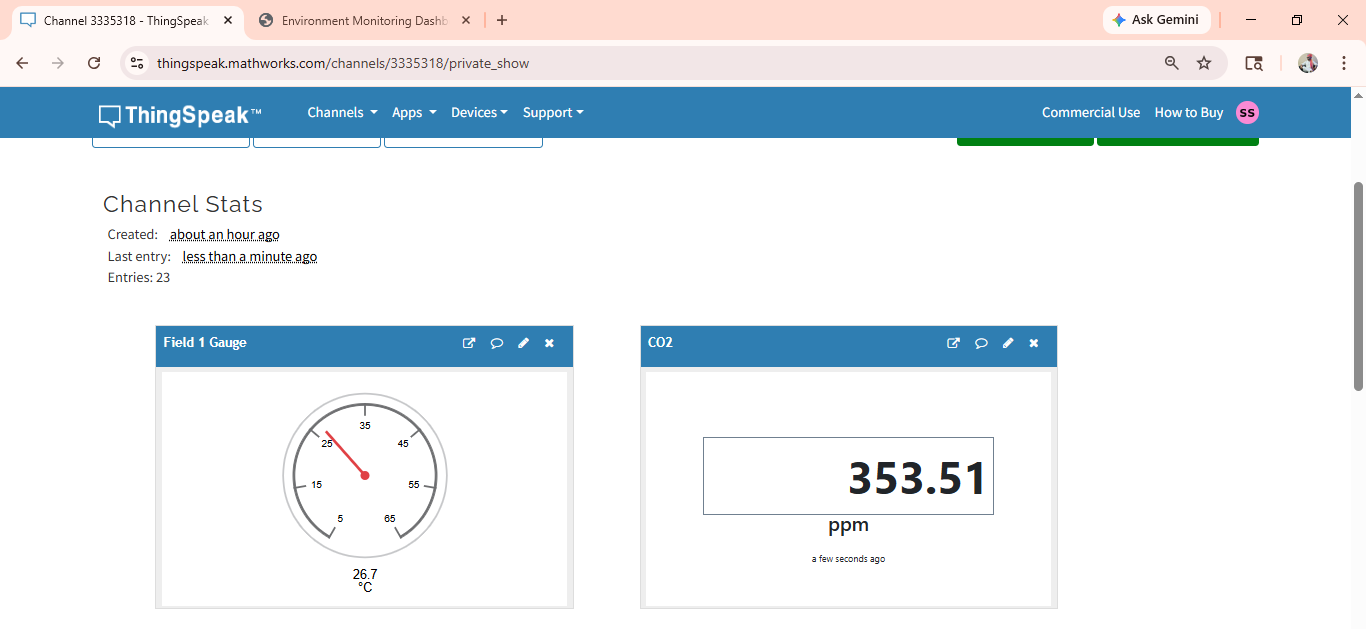
\includegraphics[width=0.90\textwidth]{ThingSpeak_Dashbaord1.png}
  \caption{ThingSpeak Channel 3335318 showing the temperature gauge and CO$_2$ display widgets with live data.}
  \label{fig:ts1}
\end{figure}

Figure~\ref{fig:ts2} presents the Field 2 (humidity) and Field 3
(CO$_2$~ppm) time-series charts, demonstrating successful end-to-end
transmission through the Raspberry Pi~3 pipeline.

\begin{figure}[tbp]
  \centering
  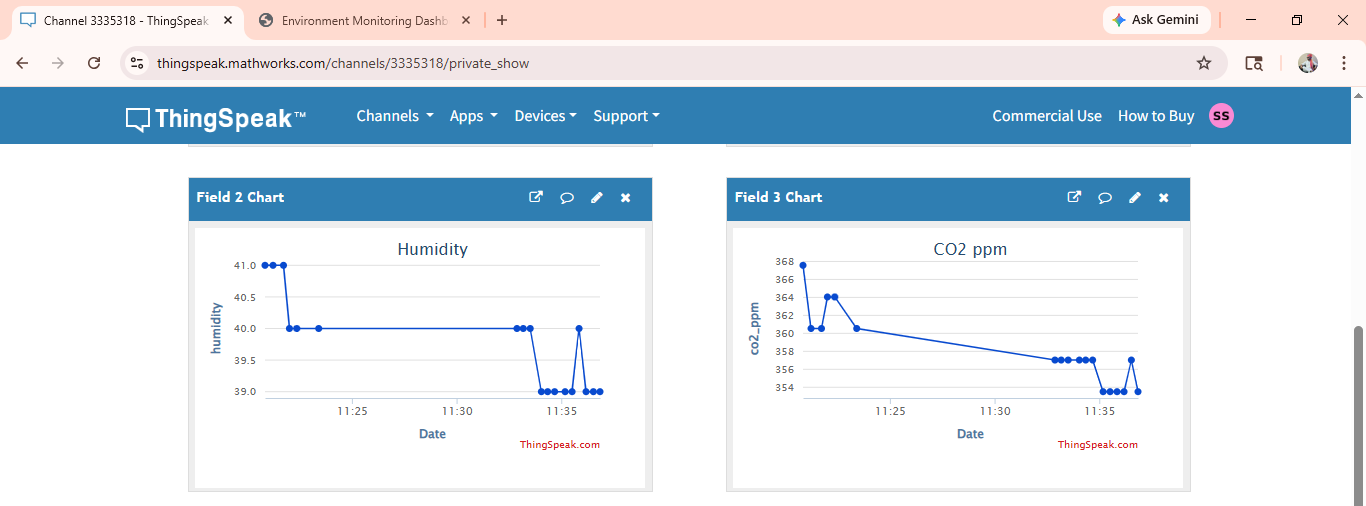
\includegraphics[width=0.90\textwidth]{ThingSpeak_Dashboard2.png}
  \caption{ThingSpeak Field 2 (humidity) and Field 3 (CO$_2$~ppm) time-series charts.}
  \label{fig:ts2}
\end{figure}

\subsection{Environmental Monitoring Session Summary}
\label{sec:envsummary}

Table~\ref{tab:envsummary} summarises the quantitative outcomes of the
two representative environmental monitoring sessions conducted during
the experimental evaluation. Both sessions confirmed stable indoor
conditions within the laboratory environment, with all readings
classified as OK throughout. The 15-second acquisition
cycle enforced by the ThingSpeak rate-limiter was maintained without
interruption in both sessions, and no write errors were recorded in
the SQLite database.

\begin{table}[tbp]
  \centering
  \caption{Summary of environmental monitoring session performance across two representative sessions.}
  \label{tab:envsummary}
  \renewcommand{\arraystretch}{1.3}
  \begin{tabular}{lcc}
    \toprule
    Metric & Session 1 (2026-04-07) & Session 2 (2026-04-10) \\
    \midrule
    Session duration (min)         & 45           & 30           \\
    Total readings acquired        & 540          & 360          \\
    Acquisition cycle (s)          & 5            & 5            \\
    Mean temperature ($^\circ$C)   & $26.5\pm0.3$ & $27.1\pm0.4$ \\
    Mean humidity (\%\,RH)        & $38\pm1$     & $39\pm1$     \\
    Mean CO$_2$ (ppm)              & $352\pm4$    & $357\pm6$    \\
    Min/Max CO$_2$ (ppm)           & 350 / 358    & 350 / 368    \\
    Alert classifications          & OK (all)     & OK (all)     \\
    SQLite write errors            & 0            & 0            \\
    Firebase push failures         & 0            & 0            \\
    ThingSpeak update rate (s)     & 15           & 15           \\
    Flask dashboard uptime         & 100\%        & 100\%        \\
    \bottomrule
  \end{tabular}
\end{table}

All CO$_2$ readings across both sessions remained below 400\,ppm,
well within the nominal OK threshold of 600\,ppm. The temperature
range of 26.5--27.1\,$^\circ$C and humidity range of 38--39\%\,RH are
consistent with comfortable indoor conditions for an air-conditioned
laboratory environment. The four parallel output channels operated
without mutual interference in both sessions, validating the threading
architecture described in Algorithm~\ref{alg:envpipeline}.

\section{Discussion}
\label{sec:disc}

The results tell a consistent story across both subsystems.

On the navigation side, the autonomous system achieved a mean tracking
error of 2.222\,cm against 16.768\,cm under manual control, an
86.75\% reduction. The worst autonomous trial (5.554\,cm RMSE) still
came in nearly 10\,cm below the best manual trial ever recorded
(14.751\,cm). The Kolmogorov--Smirnov statistic $D = 1.0$ and Cohen's
$d = 8.911$ together confirm complete distributional separation between
the two modes. The residual error of roughly 2\,cm in autonomous mode
originates primarily at corners, where the path segmentation mask
briefly loses the centroid when the tape turns sharply and the PID
derivative term cannot fully suppress the resulting correction spike.

The ONNX conversion reduced inference time from 101.6\,ms to 64.8\,ms,
a $1.57\times$ speedup, bringing throughput to 15.4\,FPS and clearing
the 15\,FPS threshold needed for stable closed-loop control. The
64.8\,ms latency per frame fits within the 50\,ms control cycle, so
the robot never had to skip a control update due to inference lag.

The PID gains ($K_p = 13.2$, $K_i = 0.0$, $K_d = 0.475$) were
determined by iterative experimental tuning on the physical robot.
The high $K_p$ compensates for the small absolute magnitude of the
normalised deviation signal, while zeroing the integral gain was a
deliberate choice to prevent drift accumulation on a
differential-drive platform with mechanical asymmetries.

For the environmental monitoring subsystem, CO$_2$ levels remained
between 350 and 368\,ppm throughout both sessions, well below the
600\,ppm threshold at which ASHRAE Standard~62.1 recommends ventilation
action. Temperature and humidity remained within occupant comfort
ranges described in the WHO Indoor Air Quality Guidelines. The linear
CO$_2$ calibration produced values consistent with the range associated
with clean, well-ventilated spaces. All four output channels operated
without mutual blocking, and the two-processor architecture maintained
independent operation of both subsystems on the shared mobile chassis
without observable cross-interference.

% ─────────────────────────────────────────────────────────
\section{Limitations of the Study}
\label{sec:lim}

Several limitations of the current framework are acknowledged. The
trajectory logging system uses simulated dead-reckoning from vision
deviation and speed command signals rather than physical wheel encoders,
so position estimates accumulate drift over a full lap and do not
constitute ground-truth position data. Experimental evaluation was
conducted on a single rectangular indoor test path under controlled
lighting; no systematic performance data was collected for
non-rectangular geometries or variable illumination conditions.
The YOLOv8n-seg model was trained exclusively on red adhesive tape
images in this specific environment and would require retraining for
a different path colour or surface type. On the sensor side, the MQ135
uses a linear calibration approximation rather than direct
electrochemical CO$_2$ measurement, which is sufficient for the
conditions tested but may exhibit calibration drift under higher
humidity or temperature variation. The ThingSpeak free tier enforces
a 15-second minimum update interval, limiting the temporal resolution
of cloud data. The system was built and validated as a single unit;
no mechanism for multi-robot coordination currently exists.